%
%%%%%%%%%%%%%%%%%%%%%%% file typeinst.tex %%%%%%%%%%%%%%%%%%%%%%%%%
%
% This is the LaTeX source for the instructions to authors using
% the LaTeX document class 'llncs.cls' for contributions to
% the Lecture Notes in Computer Sciences series.
% http://www.springer.com/lncs       Springer Heidelberg 2006/05/04
%
% It may be used as a temlpate for your own input - copy it
% to a new file with a new nam eand use it as the basis
% for your article.
%
% NB: the document class 'llncs' has its own and detailed documentation, see
% ftp://ftp.springer.de/data/pubftp/pub/tex/latex/llncs/latex2e/llncsdoc.pdf
%
%%%%%%%%%%%%%%%%%%%%%%%%%%%%%%%%%%%%%%%%%%%%%%%%%%%%%%%%%%%%%%%%%%%


\documentclass[runningheads,a4paper]{llncs}

\usepackage{amssymb}
\setcounter{tocdepth}{3}
\usepackage{graphicx}
\usepackage{amsmath}
\usepackage{booktabs}
%\usepackage{times}
\usepackage{perpage}
\usepackage{hyperref}
\MakePerPage{footnote}
\usepackage{multirow}
\usepackage{epstopdf} %converting to PDF
\usepackage{tikz}
\usetikzlibrary{arrows,patterns,automata,backgrounds,decorations,fit,petri,positioning,petri,shapes,calc}
\usepackage[caption=false]{subfig}
\usepackage{url}
\usepackage{wrapfig}

\usepackage{color}
\usepackage{xcolor}
\definecolor{dkgreen}{rgb}{0,0.6,0}
\definecolor{gray}{rgb}{0.5,0.5,0.5}
\definecolor{mauve}{rgb}{0.58,0,0.82}
\definecolor{background}{HTML}{EEEEEE}
\definecolor{delim}{RGB}{20,105,176}
\colorlet{punct}{red!60!black}
\colorlet{numb}{magenta!60!black}

\usepackage{listings}
\lstset{
	%language=python,                % the language of the code
	language=C++,
	basicstyle=\footnotesize,        % the size of the fonts that are used for the code
	%numbers=left,                   % where to put the line-numbers
	%numberstyle=\footnotesize,      % the size of the fonts that are used for the line-numbers
	numberstyle=\tiny\color{gray},
	stepnumber=1,                    % the step between two line-numbers. If it's 1, each line
	% will be numbered
	numbersep=5pt,                   % how far the line-numbers are from the code
	backgroundcolor=\color{white},   % choose the background color. You must add \usepackage{color}
	showspaces=false,                % show spaces adding particular underscores
	showstringspaces=false,          % underline spaces within strings
	showtabs=false,                  % show tabs within strings adding particular underscores
	frame = lines,
	%frame=single,                   % adds a frame around the code
	rulecolor=\color{black},		   % if not set, the frame-color may be changed on line-breaks within
	% not-black text (e.g. commens (green here))
	tabsize=2,                       % sets default tabsize to 2 spaces
	captionpos=b,                    % sets the caption-position to bottom
	breaklines=true,                 % sets automatic line breaking
	breakatwhitespace=false,         % sets if automatic breaks should only happen at whitespace
	%title=\lstname,                 % show the filename of files included with \lstinputlisting;
	% also try caption instead of title
	% also try caption instead of title
	keywordstyle=\color{blue},       % keyword style
	commentstyle=\color{dkgreen},    % comment style
	stringstyle=\color{mauve},       % string literal style
	escapeinside={\%*}{*)},          % if you want to add a comment within your code
	morekeywords={*,game, fun}       % if you want to add more keywords to the set
}

% params for json visualization, tacken from https://tex.stackexchange.com/questions/83085/how-to-improve-listings-display-of-json-files
\lstdefinelanguage{json}{
	basicstyle=\footnotesize\ttfamily,
	numbers=left,
	numberstyle=\scriptsize\color{gray},
	stepnumber=1,
	numbersep=8pt,
	showstringspaces=false,
	breaklines=true,
	frame=lines,
	backgroundcolor=\color{background},
	literate=
	*{0}{{{\color{numb}0}}}{1}
	{1}{{{\color{numb}1}}}{1}
	{2}{{{\color{numb}2}}}{1}
	{3}{{{\color{numb}3}}}{1}
	{4}{{{\color{numb}4}}}{1}
	{5}{{{\color{numb}5}}}{1}
	{6}{{{\color{numb}6}}}{1}
	{7}{{{\color{numb}7}}}{1}
	{8}{{{\color{numb}8}}}{1}
	{9}{{{\color{numb}9}}}{1}
	{:}{{{\color{punct}{:}}}}{1}
	{,}{{{\color{punct}{,}}}}{1}
	{\{}{{{\color{delim}{\{}}}}{1}
	{\}}{{{\color{delim}{\}}}}}{1}
	{[}{{{\color{delim}{[}}}}{1}
	{]}{{{\color{delim}{]}}}}{1},
}

\usepackage{times}
\addtolength{\topmargin}{-2\baselineskip}
\addtolength{\textheight}{3\baselineskip}

\urldef{\mailsa}\path|ilya.verenich@qut.edu.au|
\urldef{\mailsb}\path|{stanislav.myshkovski,marlon.dumas,f.m.maggi}@ut.ee|
\urldef{\mailsc}\path|{simon.raboczi,marcello.larosa}@unimelb.edu.au|

\newcommand{\keywords}[1]{\par\addvspace\baselineskip
\noindent\keywordname\enspace\ignorespaces#1}

\begin{document}

\mainmatter  % start of an individual contribution

% first the title is needed
\title{Predictive Process Monitoring in Apromore}

% a short form should be given in case it is too long for the running head
\authorrunning{Verenich et al.}
\titlerunning{Predictive Process Monitoring in Apromore}

% the name(s) of the author(s) follow(s) next
%
% NB: Chinese authors should write their first names(s) in front of
% their surnames. This ensures that the names appear correctly in
% the running heads and the author index.
%
\author{Ilya Verenich\inst{1,2}  \and Stanislav M\~{o}\v{s}kovski\inst{2} \and Simon Raboczi\inst{3} \and  Marlon Dumas\inst{2}  \and\\Marcello La Rosa\inst{3} \and Fabrizio Maria Maggi\inst{2}}

\institute{Queensland University of Technology, Australia\\
\mailsa
\and University of Tartu, Estonia\\
\mailsb
\and University of Melbourne, Australia\\
\mailsc
}

%
% NB: a more complex sample for affiliations and the mapping to the
% corresponding authors can be found in the file "llncs.dem"
% (search for the string "\mainmatter" where a contribution starts).
% "llncs.dem" accompanies the document class "llncs.cls".
%

%\toctitle{Predictive Process Monitoring Using LSTM}
%\tocauthor{Authors' Instructions}
\maketitle


\begin{abstract}
This paper discusses the integration of Nirdizati, a tool for predictive process monitoring, into the Web-based process analytics platform Apromore. Through this integration, Apromore's users can use event logs stored in the Apromore repository to train a range of predictive models, and later use the trained models to predict various performance indicators of running process cases from a live event stream. For example, one can predict the remaining time or the next events until case completion, the case outcome, or the violation of compliance rules or internal policies. %For example, in a claim handling process, the tool can predict if a claim decision will be made on time or late.
%Based on these predictions, process workers and operational managers can act proactively to resolve or mitigate potential process performance violations.
%The target audience of this demonstration includes process mining researchers as well as practitioners interested in exploring the potential of process monitoring.
%In this paper, we present a prototype of a web-based application for predictive process monitoring that can be used by process participants and operational managers to predict the future development of a currently running process execution.
%The implemented solution, named \emph{Nirdizati}, is a configurable full-stack web application that supports users in selecting the preferred prediction methods from a list of implemented algorithms and enables the continuous prediction of various measures of interest at runtime.
The predictions can be presented graphically via a dashboard that offers multiple visualization options, including a range of summary statistics about ongoing and past process cases. They can also be exported into CSV for periodic reporting or to be visualized in third-parties business intelligence tools. Based on these predictions, operations managers may identify potential issues early on, and take remedial actions in a timely fashion, e.g.\ reallocating resources from one case onto another to avoid that the case runs overtime. %The target audience of this demonstration includes process mining researchers as well as practitioners interested in exploring the potential of predictive process monitoring.

\keywords{Process mining, predictive monitoring, business process, machine learning}
\end{abstract}


\section{Introduction} \label{sec:intro}
\emph{Predictive Process Monitoring} is an emerging paradigm based on the continuous generation of predictions about the future values of user-specified performance indicators of a currently running process execution \cite{PredictiveMonitoring}.
%and recommendations on what activities to perform and what input data values to provide, so that the likelihood of violation of business constraints is minimized. % and violations can be avoided.
In this paradigm, a user defines the type of predictions they are interested in and provides a set of historical execution traces. Based on the analysis of these traces, the idea of predictive monitoring is to continuously provide the user with predictions and estimated values of the performance indicators. Such predictions generally depend both on: (i) the sequence of activities executed in a given case; and (ii) the values of data attributes after each activity execution in the case.

%As an example, consider a doctor who needs to choose the most appropriate therapy for a patient. Historical data referring to patients with similar characteristics can be used to predict what therapy will be the most effective one and to advise the doctor accordingly. Meanwhile, in the context of a business process for managing loan applications, the applicant can be advised on the combinations of the loan amount and the length period for the loan that are the most likely to lead to acceptance of the application, given contextual information about the application and the personal data of the applicant (e.g., age, salary, etc.).
There are many scenarios where it is useful to have reliable predictions. For example, in a purchase-to-pay business process, a customer can be advised about the estimated supply date. In case this date violates service-level agreement (SLA), preemptive actions can be taken by the supplier to prevent or mitigate the delay.

A range of approaches have been proposed in the literature to tackle common predictive process monitoring tasks. A recent survey of this field \cite{Chamorro2017} identified 39 distinct proposals (excluding subsumed ones) targeting time-related predictions, future path predictions and case outcome predictions.
However, these approaches have largely remained in the academic domain and have not been widely applied in real-time scenarios where users require a continuous predictive support.

To fill this gap, last year we started the \emph{Nirdizati} open-source project, aimed at developing a Web-based tool for the predictive monitoring of business processes \cite{Jorbina2017}. This paper documents a major revision of the project. Following state of the art in predictive processing monitoring and numerous feedback we received from prospective users, we have redesigned the user interface, technology stack and predictive techniques behind the tool. Furthermore, both training and runtime functionality have been integrated into the process analytics platform Apromore.\footnote{\url{http://apromore.org}}

%In this paper, we present the integration of Nirdizati into the process analytics platform Apromore. Nirdizati is a pioneering Web-based predictive monitoring tool, which is able to fill this gap between research and practice, by providing business analysts with a highly flexible instrument for the selection, generation and analysis of different predictive models, and end-users with continuous runtime predictions.


%\vspace{-\baselineskip}
\begin{figure}[t]%[H]
	\centering
	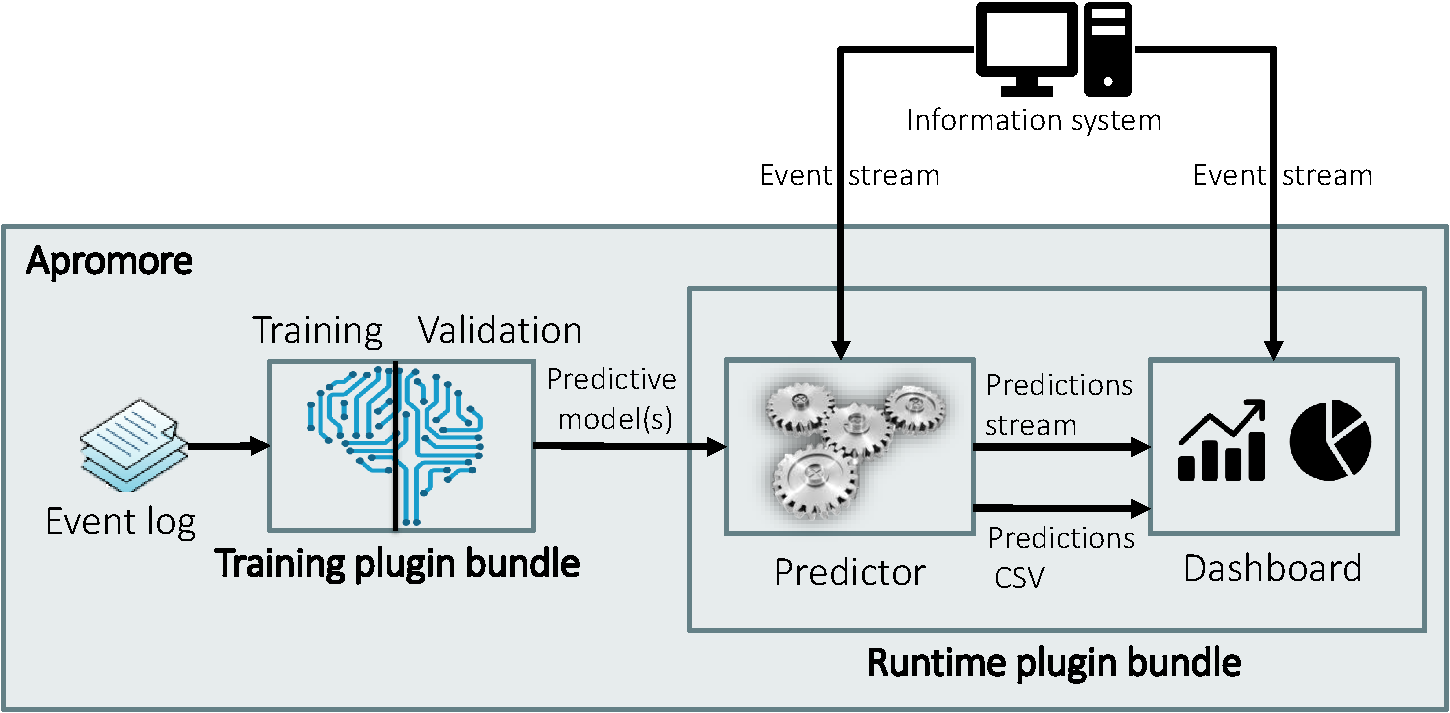
\includegraphics[width=0.7\textwidth]{img/nirdizati-overall.pdf}
	\caption{High-level architecture of the predictive monitoring functionality of Apromore.}
	\label{fig:nirdizati-overall}
\end{figure}
%\vspace{-\baselineskip}

The two core components of Nirdizati, namely \textit{Training} and \textit{Runtime}, have been integrated as two bundles (i.e.\ sets) of plugins into Apromore (\figurename~\ref{fig:nirdizati-overall}). The Training plugin bundle takes as input a business process event log stored in the Apromore repository, and produces one or more predictive models, which can then be deployed to the runtime predictive monitoring environment. Once a model is deployed, the Runtime plugin bundle listens to a stream of events coming from an information system supporting the process, or produced by replaying an event log stored in the repository, and creates a stream of predictions. These predictions can then be visualized in a Web dashboard or exported into a CSV (comma-separated value) file for periodic reporting and to be used within third-party business intelligence tools.
%Nirdizati consists of two components: Nirdizati Training and Nirdizati Runtime (Figure~\ref{fig:nirdizati-overall}). Nirdizati Training takes as input a business process event log and produces a predictive model. This model can then be deployed in Nirdizati Runtime. Once a model is deployed, Nirdizati Runtime listens to a stream of events related to a business process, and produces a stream of predictions. These predictions are then visualized in a continuously updated web dashboard.

\section{Apromore Platform}
Apromore is a Web-based advanced process analytics platform, developed by the business process management (BPM) community under an open-source initiative. Apromore was originally conceived as an advanced process model repository. However, today it offers a wide range of features which go beyond those for managing large process model collections, and include a variety of state-of-the-art process mining techniques. These are techniques for the automated discovery of BPMN models, for the conformance checking of BPMN models against event logs, the replaying of event logs on top of BPMN models, the detection and characterization of process drifts from event logs, the visual analysis of process performance, and many others. 

All these features are exposed through a Web portal, and organized according to the phases of the BPM lifecycle: discovery, analysis, redesign, implementation and monitoring \cite{Dumas2018}. These features can also be accessed as external Web services by third-party BPM software environments, such as ProM (for process mining) and WoPeD (for process modeling and verification).

From a technology viewpoint, Apromore relies on four core technologies: Spring, ZK, OSGi and Eclipse Virgo. Spring provides a simplified management of Java-based enterprise applications through the use of Java annotations and XML configurations. ZK is an AJAX framework used for Apromore's main Web interface (the \emph{Portal}). OSGi provides a flexible framework for managing component dependencies through plugin bundles. Finally, Eclipse Virgo is a Web server based on the OSGi component model.

To equip Apromore with predictive process monitoring capabilities, we have wrapped the two core components of Nirdizati into two OSGi plugin bundles for Apromore: Training and Runtime. Each bundle is a set of OSGi plugins which encapsulate the logic or the user interface (UI) of the various functions offered by Nirdizati. For example, the runtime predictor is a logic plugin, while the runtime dashboard is a portal plugin (UI). These two bundles are accessible from the Monitoring menu of the Apromore Portal (see Figure~\ref{fig:apromore-menus}). One can select an event log stored in the repository, and use it to train, tune and test a variety of predictive models, by launching the training plugin bundle. Next, the runtime bundle can be used to stream an event log from the repository, or hook into a live external stream, to generate predictions as process cases unfold.    

\begin{figure}[t!]%[H]
	\centering
	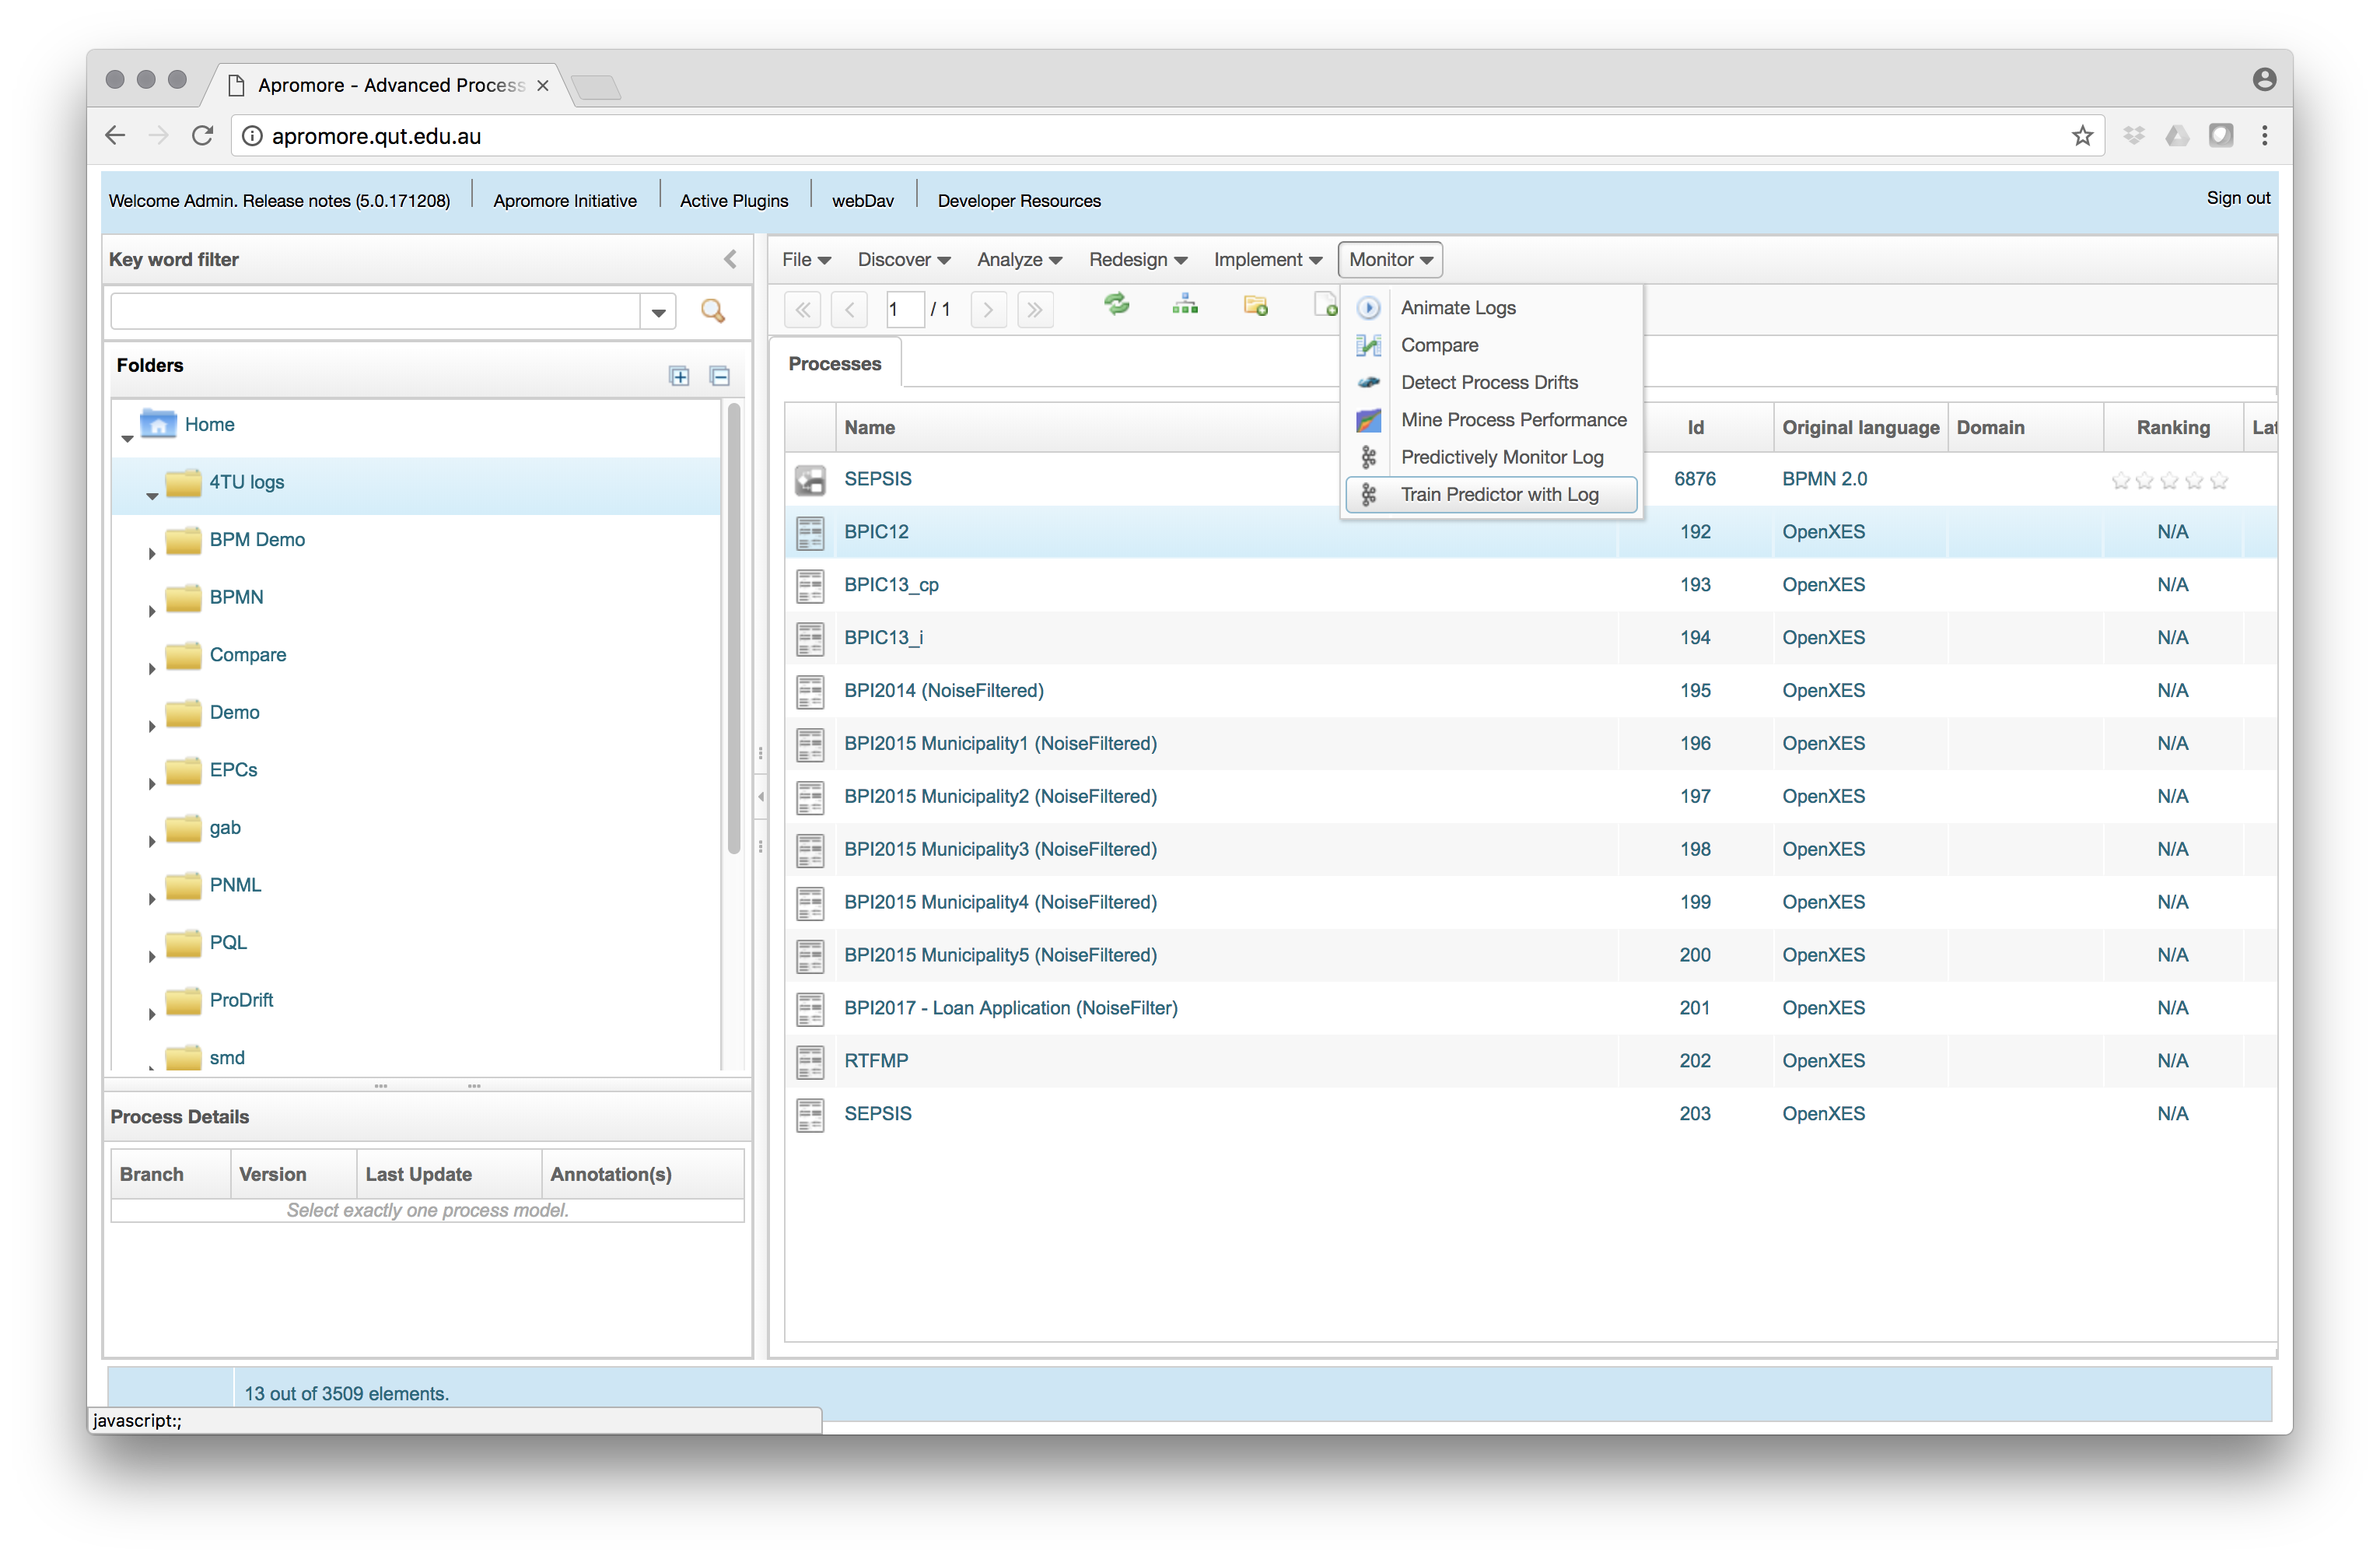
\includegraphics[width=\textwidth]{img/apromore-menus}
	%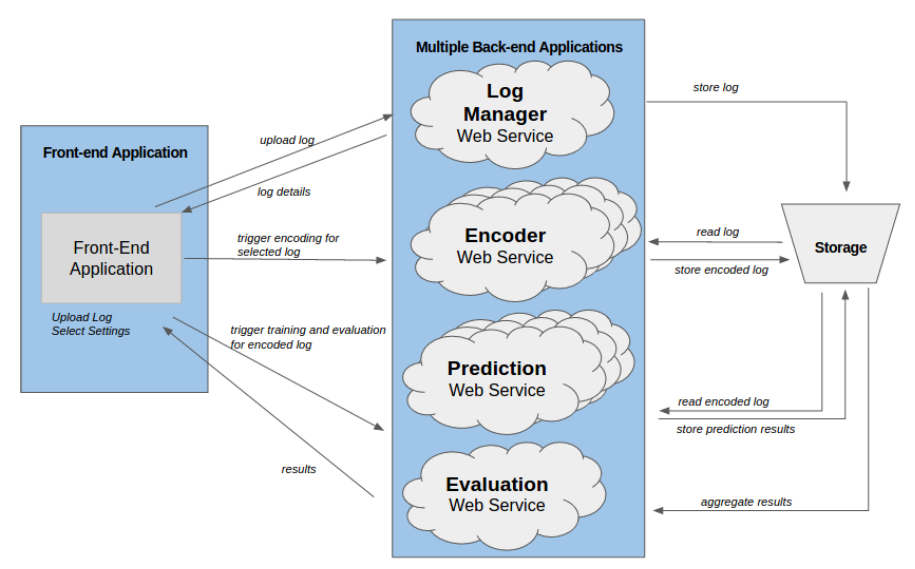
\includegraphics[width=0.7\textwidth]{img/nirdizati-training}
	\vspace{-2\baselineskip}
	\caption{Apromore's Portal with predictive monitoring functionality highlighted.}
	\label{fig:apromore-menus}
	\vspace{-0.5\baselineskip}
\end{figure}

In the next sections, we introduce a working example and use this to describe the functionality of the training and runtime plugins in detail.



\section{Running Example}
As a running example, throughout this paper we will consider a purchase-to-pay process of an IT vendor. The process starts with lodging a purchase order and ends when requested goods have been supplied. 

For use with the Training plugin bundle, we extracted an event log of completed purchased orders, while ongoing orders were fed into the Runtime plugin bundle to make predictions for them. The corresponding event log contains a number of case attributes, such as the total cost of the order, supplier identifier, supplier location, delivery type and the target supply date. Moreover, each event contains identifier of an employee who performed it.

In this process, stakeholders are interested in predicting four variables:
\begin{itemize}
	\item \emph{Late supply}. It is a boolean variable indicating whether or not the case will be closed before the supply date of that case.
	\item \emph{Delay Rank} indicating the degree of potential delay, namely ``Just in case'', ``Mild'', ``Moderate'', ``Severe''.
	\item \emph{Next activity} indicating which activity will be performed right after the current one.
	\item \emph{Remaining time} until case completion.
\end{itemize}

In order to make more accurate predictions, we performed some basic feature engineering before feeding the log into Apromore. For example, to take into account resource contention, we added the number of currently open cases as an event attribute. Furthermore, instead of the absolute target supply date, we used the number of days relative to the case start date. Intuitively, if this number is lower, there exists a higher probability of missing the deadline (Late Supply).

\section{Training Plugin Bundle} \label{sec:training}
%\begin{wrapfigure}
%	{r}{0.6\textwidth}
%%\begin{figure}[t]
%\vspace{-2\baselineskip}
%	\centering
%	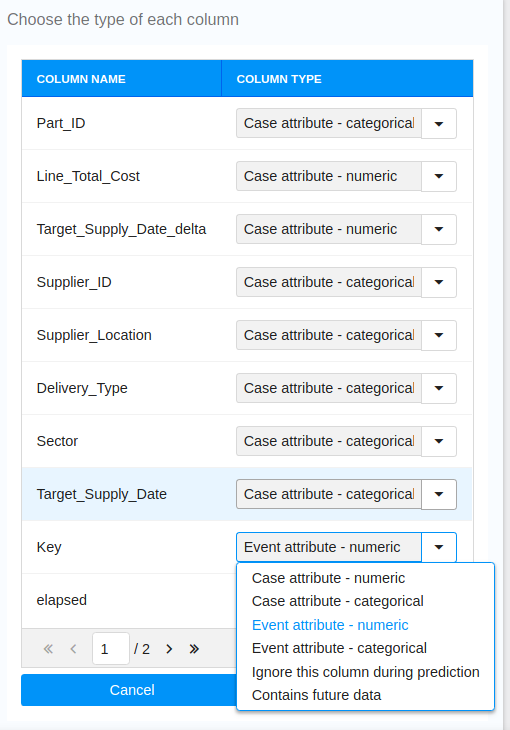
\includegraphics[width=0.4\textwidth]{img/attribute-selector}
%	\caption{Attribute type selector in the training plugin.}
%	\label{fig:attribute-selector}
%	\vspace{-2\baselineskip}
%%\end{figure}
%\end{wrapfigure}
The Training plugin bundle provides several algorithms for generating predictive models suitable for different types of predictions. Specifically, it is able to build models for predicting remaining time, the next activity to be performed, whether a case will exceed a specified duration threshold, as well as various static case attributes, for example, the total cost of the order.
%
To this aim, the Training bundle involves two phases: a training and a validation phase. In the former, one or more predictive models are fitted; in the latter, their suitability to the specific dataset is evaluated, so as to support the user in selecting the predictive model that ensures the best results.

\begin{figure}[t!]%[H]
	\centering
	 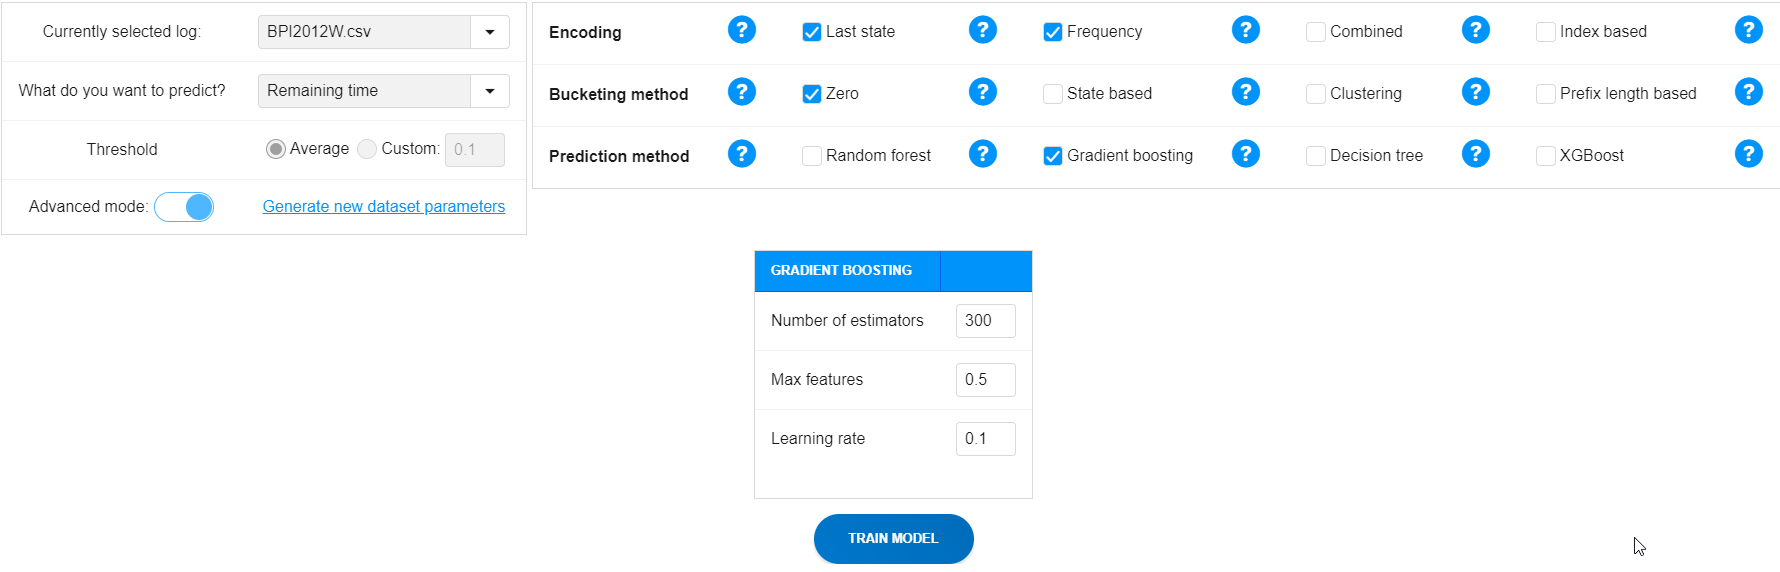
\includegraphics[width=\textwidth]{img/nirdizati-frontend2}
	%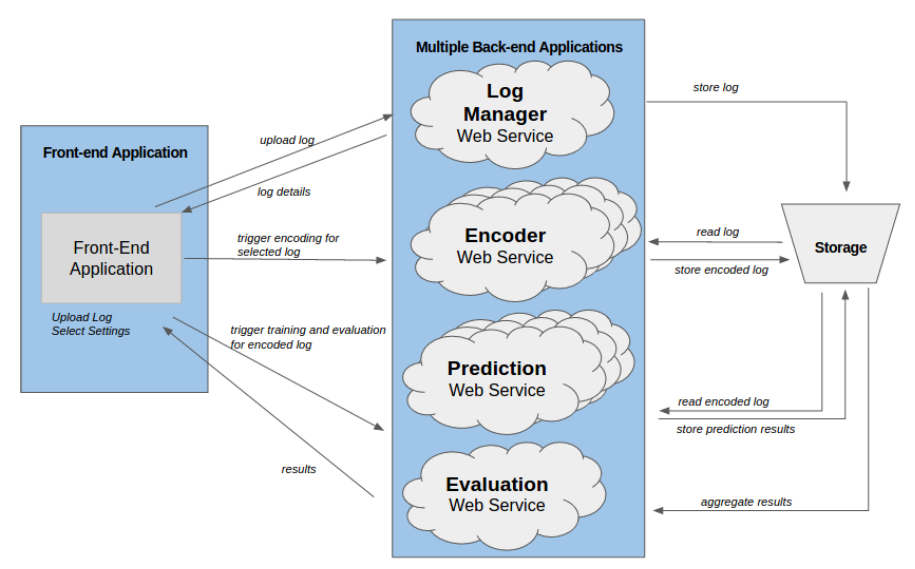
\includegraphics[width=0.7\textwidth]{img/nirdizati-training}
	\caption{Training configuration screen.}
	\label{fig:nirdizati-frontend}
	\vspace{-0.5\baselineskip}
\end{figure}
\begin{figure}[b!]%[H]
	\centering
	 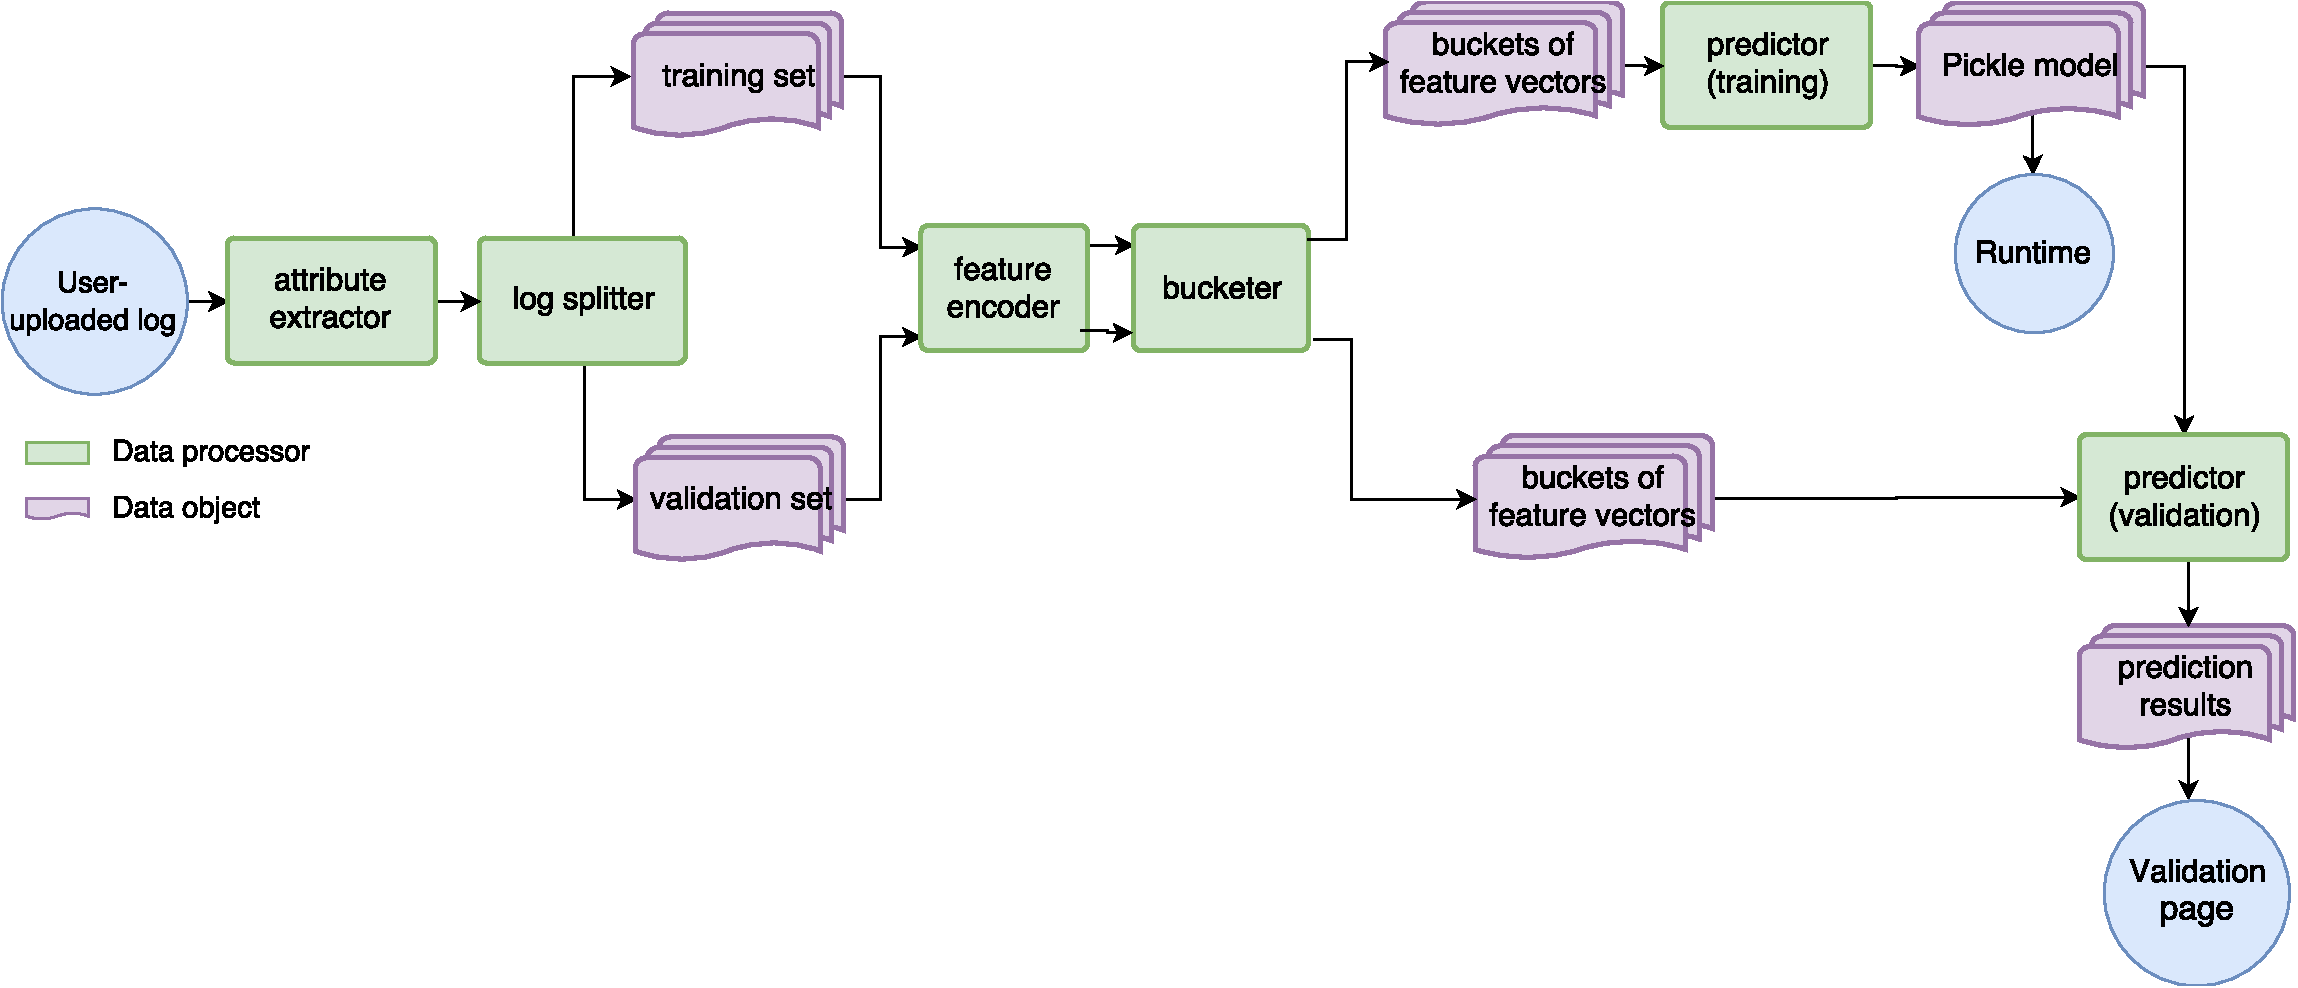
\includegraphics[width=\textwidth]{img/training-dataflow}
	%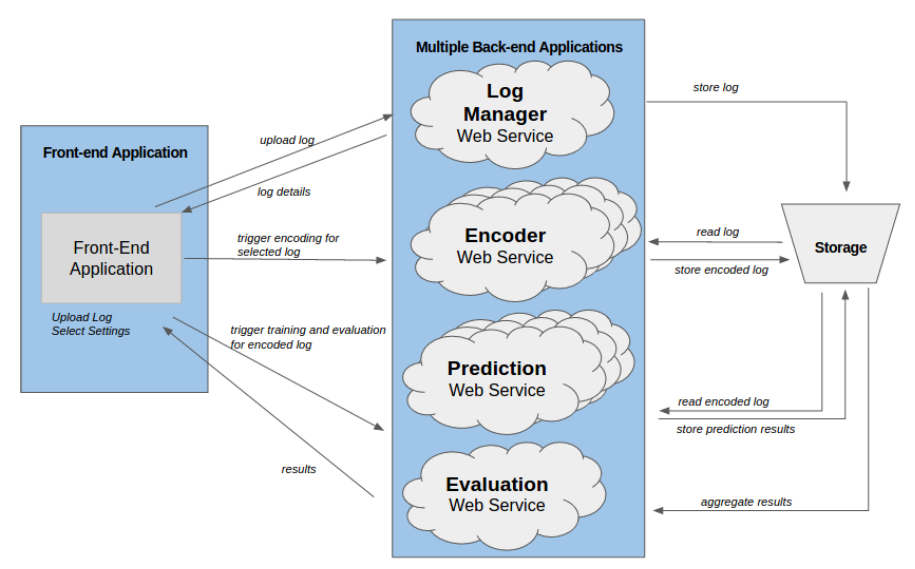
\includegraphics[width=0.7\textwidth]{img/nirdizati-training}
	\caption{High-level data flow diagram of the Training plugin bundle.}
	\label{fig:nirdizati-training}
	\end{figure}
%\vspace{-2\baselineskip}
The Training bundle is composed of a front-end application (\figurename~\ref{fig:nirdizati-frontend}), which allows users to select the prediction methods
and to assess the goodness-of-fit of the built models, and a back-end application  for the actual training and validation. From the data flow perspective, the back-end application performs several tasks shown in \figurename~\ref{fig:nirdizati-training}.

Firstly, when a user uploads their log, the tool extracts and categorizes data attributes of the log into static case attributes and dynamic event attributes. To this end, for each attribute in the log, we check whether it changes throughout the case lifetime. On the other hand, each attribute needs to be designated as either numeric or categorical. 

%\begin{lstlisting}[float,floatplacement=H,language=json,firstnumber=1,caption={Example training configuration file},captionpos=b,label={lst:training-config}]
%{
%"case_id_col":"Line_ID",
%"activity_col":"Activity_Name",
%"timestamp_col":"Activity_End_Time",
%"static_cat_cols":["Supplier_ID","Supplier_Location","Delivery_Type","Sector"],
%"dynamic_cat_cols":["Employee_ID","weekday"],
%"static_num_cols":["Line_Total_Cost","Target_Supply_Date_delta"],
%"dynamic_num_cols":["elapsed","timesincelastevent","open_cases"],
%"ignore":["Activity_Start_Time","hour","Milestone","Key","Target_Supply_Date","Part_ID"],
%"future_values":["Late_Supply","Delay_Rank"],
%}
%\end{lstlisting}

In order to do that, we count the number of unique levels in the values of each attribute and if it less than a certain threshold, we decide the attribute to be categorical, otherwise it is numeric. These procedures are performed automatically upon the log uploading. Nevertheless, the user is given an option to override the automatic attribute definitions. Proper attribute categorization ensures best training data quality. 
The resulting definitions are saved in a configuration file in a JSON format (Fig.~\ref{fig:listing}). Secondly, the log is internally split into training and validation set in a 80-20 proportion. The former is used to train the model, while the latter is used to evaluate the predictive power of the model. Next, all traces of a business process need to be represented as fixed-size feature vectors in order to train a predictive model. To this end, several encoding techniques were proposed in \cite{Leontjeva2015} and further refined in \cite{Teinemaa2017}, out of which we support four, namely last state encoding, frequency (aggregation) encoding, combined encoding and lossless index-based encoding. 
\begin{figure}[htp!]%[H]
	\centering
	 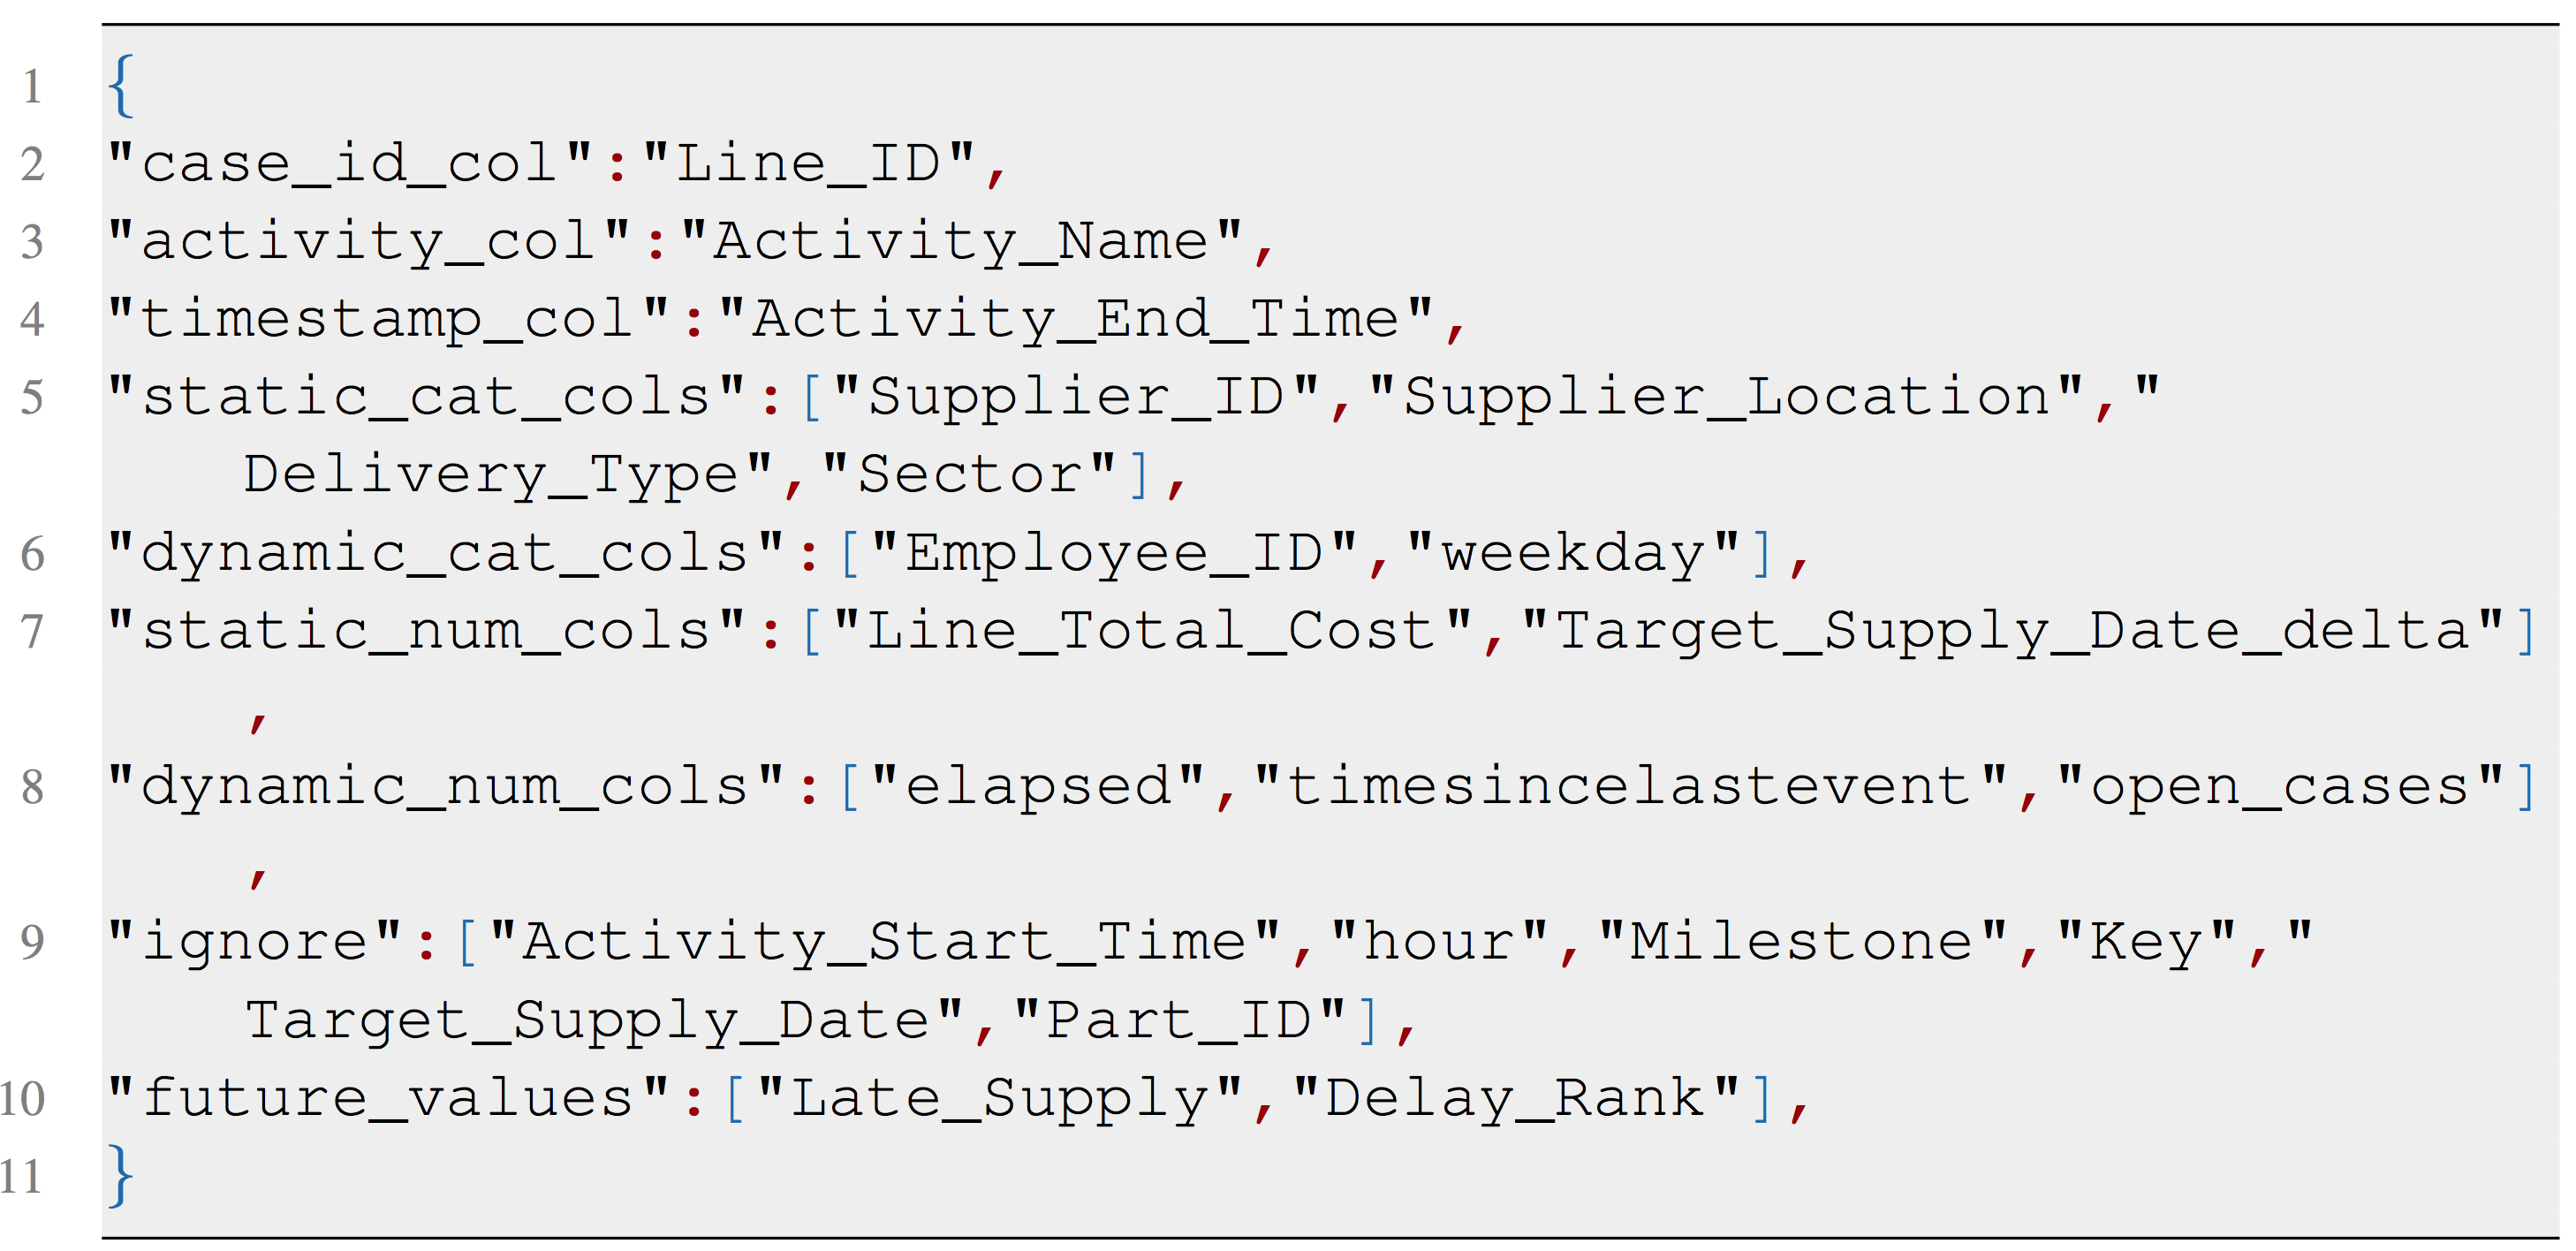
\includegraphics[width=.7\textwidth]{img/Listing}
	%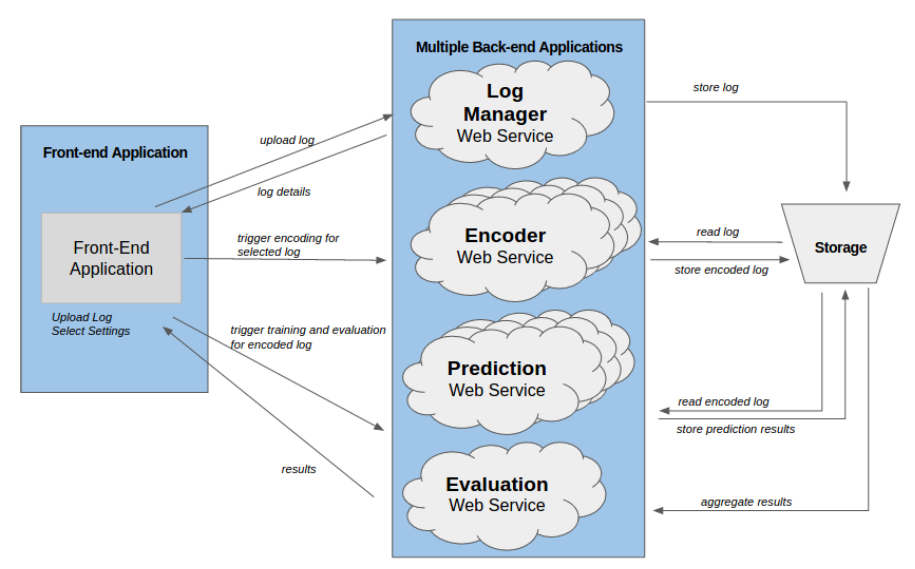
\includegraphics[width=0.7\textwidth]{img/nirdizati-training}
	\caption{Example training configuration file.}
	\label{fig:listing}
	\vspace{-\baselineskip}
\end{figure}

While some of existing predictive process monitoring approaches train a single classifier on the whole event log, others employ a multi-classifier approach by dividing the prefix traces in the historical log into several buckets and fitting a separate classifier for each such bucket. At run-time, the most suitable bucket for the ongoing case is determined and the respective classifier is applied to make a prediction. Various bucketing types have been proposed and described in detail in \cite{Teinemaa2017}. The Training bundle supports four types of bucketing: zero bucketing (i.e. fitting a single classifier), state-based bucketing, clustering-based bucketing and prefix length-based bucketing.

For each bucket of feature vectors, we train a predictive model using one of four supported machine learning techniques: decision tree, random forest, gradient boosting and extreme gradient boosting (XGBoost). For each technique, a user may manually enter the values of the most important hyperparameters. For example, when fitting a gradient boosting model, a user may choose the number of weak learners (trees), the number of features to be used for each split and the learning rate.

In order to accommodate users with varying degrees of expertise in machine learning and predictive process monitoring, the plugin bundle offers two training modes -- basic and advanced. By default, the basic mode is activated wherein a user only needs to choose the log and prediction target. If the prediction target is based on the logical rule -- whether the case duration will exceed the specified threshold, a user is also invited to key in the threshold value. For all the other settings -- bucketing method, encoding method and prediction method and its hyperparameters -- the default values which usually achieve the best prediction accuracy will be used. Experienced users may switch the advanced mode toggle and manually choose bucketing, encoding and prediction method settings or any sensible combination thereof. The latter is especially useful when a user wants to train and compare multiple models, e.g. using various sequence encoding methods.

The status of the trained models can be verified using the collapsible drawer in the right-hand corner. Upon the training completion, a serialized Python object in the pickle format is produced. It describes a trained predictive model and includes:

\begin{itemize}
	\item Configuration parameters of the predictors (whether it is a classifier or a regressor, what learning algorithm it uses)
	\item Definition of each column of the event log (static or dynamic, numeric or categorical). This information allows the Runtime plugin bundle to construct a feature vector from a given partial trace.
	\item The bucketing function, which given an input sample, allows us to determine which classifier/regressor should be used. Unless a zero bucketing is used, the pickle file has a different classifier/regressor per bucket.
	\item For each bucket, the trained model, ready to be taken as input by the selected classification algorithm, e.g. in the case of decision trees, the whole tree representation.
\end{itemize}

The predictive power of the trained model(s) can be evaluated on a held-out validation set. By default, a user will see the average accuracy across all partial traces after a certain number of events have completed. This evaluation method was also used in \cite{Leontjeva2015} and \cite{Teinemaa2017}. For classification tasks (e.g. prediction of Late Supply and Delay Rank), a user can choose which metrics to plot among accuracy score, F1 score and logarithmic loss. For regression tasks (e.g. remaining time), a user can choose between mean absolute error, either raw or normalized, and root mean square error. The accuracy of a particular model can be visually compared with that of other models trained for the same log and the same prediction target (Figure~\ref{fig:training-evaluation}). Additionally, one can check a scatterplot of predicted vs. actual values (for regression tasks) or a confusion matrix (for classification tasks) and assess the relative importance of each feature for the chosen predictor.

\begin{figure}[t]
	\centering
	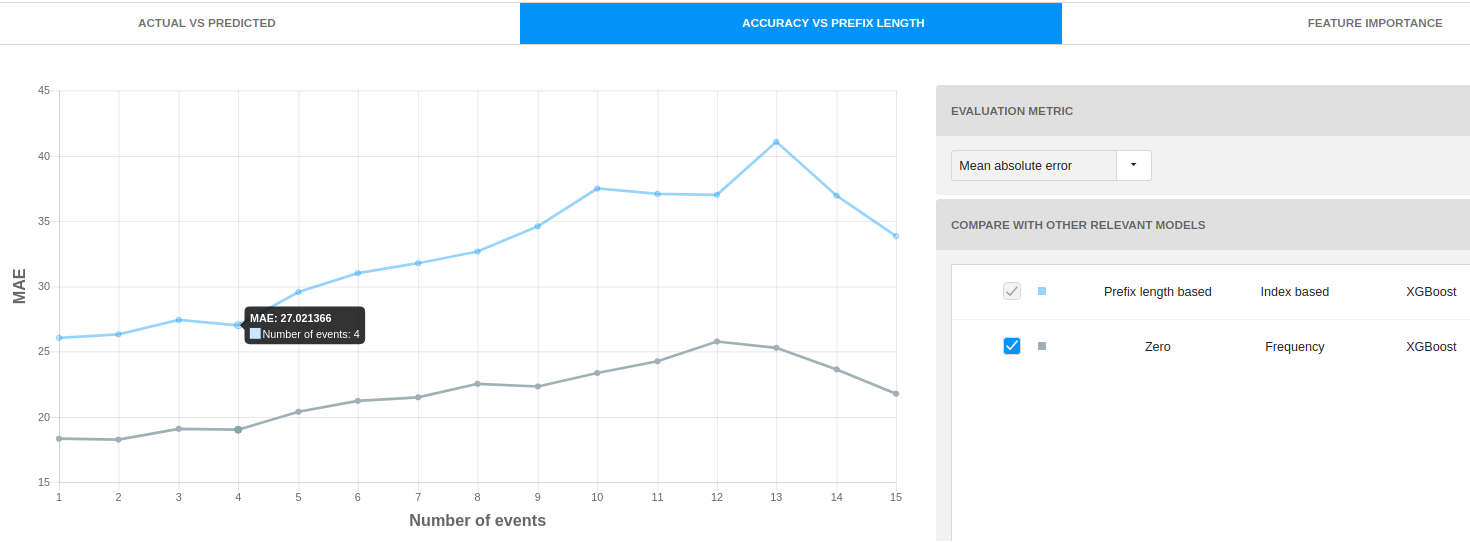
\includegraphics[width=0.93\textwidth]{img/training-evaluation}
	\caption{Model validation page of the Training plugin bundle.}
	\label{fig:training-evaluation}
\end{figure}
%\vspace{-\baselineskip}

\section{Runtime Plugin Bundle} \label{sec:runtime}
Once the predictive models have been created, they can be deployed to the Runtime predictive monitoring environment of Apromore, to make predictions on ongoing cases. The Runtime plugin bundle can be used to stream an event log from the repository, or hook into an external stream. Either way, the input stream is transformed into a stream of predictions which is visualized in a Web-based dashboard. The transformation is implemented using the dataflow pipeline in \figurename~\ref{fig:dfd_0}.
\vspace{-.5\baselineskip}
\begin{figure}[htp!]
	\centering
	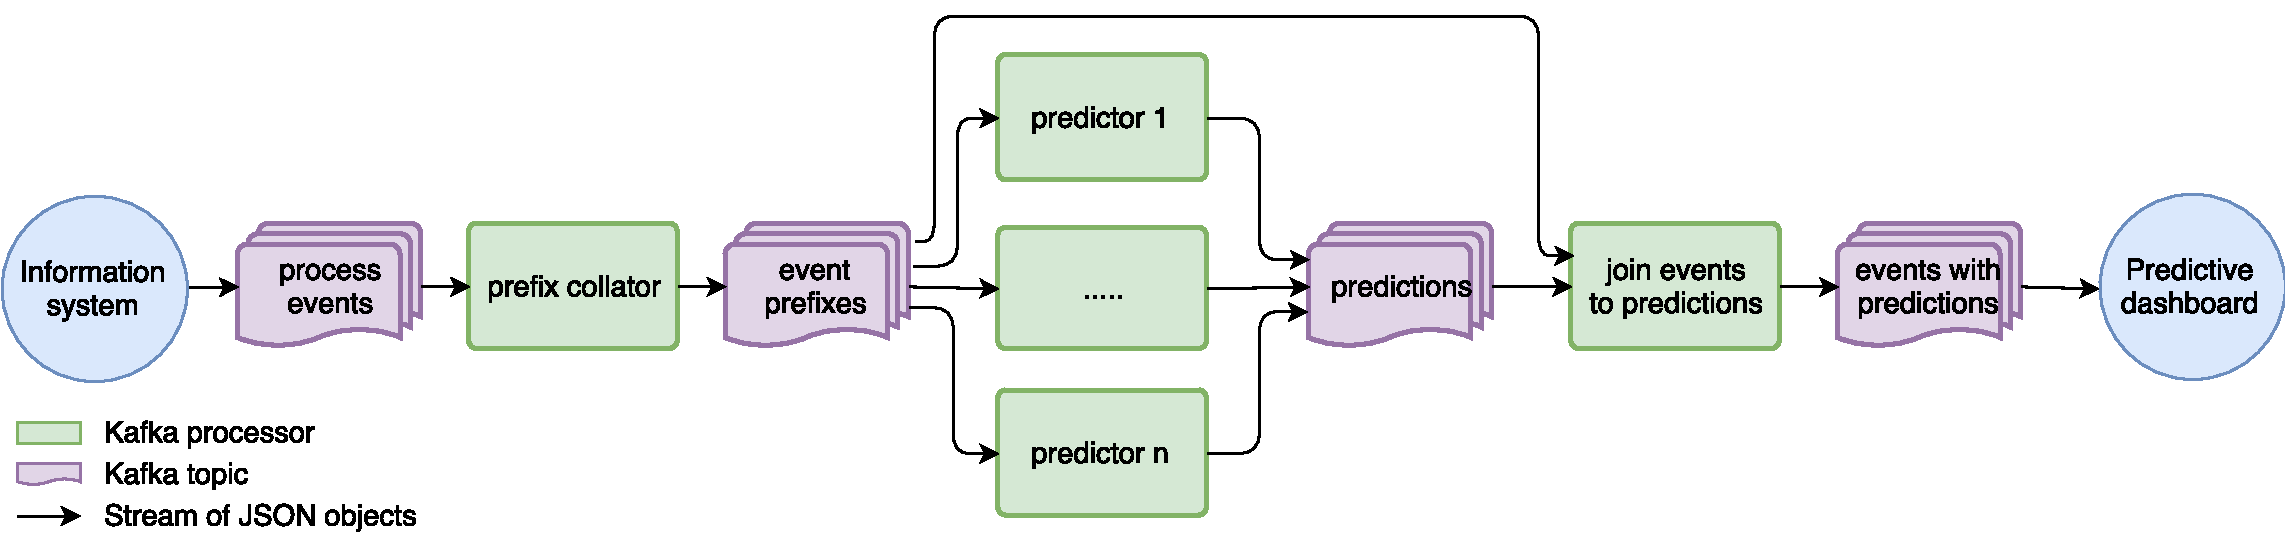
\includegraphics[width=\textwidth]{img/runtime-dataflow}
	\caption{High-level data flow diagram of the Runtime plugin bundle.}
	\label{fig:dfd_0}
\end{figure}
\vspace{-.5\baselineskip}

The pipeline is built on top of the open-source Apache Kafka stream processing platform.\footnote{\url{https://kafka.apache.org}} The ``predictor'' components of the pipeline are the predictive models from the Training plugin bundle. The ``topic'' components are network-accessible queues of JSON messages with publisher/subscriber support. This allows the computationally intense work of the predictors to be distributed across a cluster of networked computers, providing scalability and fault-tolerance.
The ``collator'' component accumulates the sequence of events-to-date for each case, such that the prediction is a stateless function of the trained predictive model and of the case history.  This statelessness is what allows the predictors to be freely duplicated and distributed.  The ``joiner'' component composes the original events with the various predictions, ready for display on the dashboard.

The dashboard provides a list of both currently ongoing cases (colored in gray) as well as completed cases (colored in green), as shown in \figurename~\ref{fig:nirdizati-runtime}. For each case, it is also possible to visualize a range of summary statistics including the number of events in the case, its starting time and the time when the latest event in the case has occurred. For the ongoing cases, the Runtime plugin bundle provides the predicted values of the performance indicators the user wants to predict. For completed cases, instead, it shows the actual values of the indicators. In addition to the table view, the dashboard offers other visualization options, such as pie charts for case outcomes and bar charts for case durations. It is also possible to export the predictions in a CSV file, for periodic reporting and for importing into third-party business intelligence tools.

%The upper panel shows aggregated process indicators, such as the number of currently running and so far completed cases, the number of occurred events, average number of events per case and average case duration.

%Nirdizati also allows monitoring multiple event streams simultaneously. The drop-down list in the top right corner allows a user to switch the stream. When a user switches to another process, all information in the dashboard is updated automatically. At the same time, each user can choose which process to monitor without interfering with others.

%The Outcomes tab provides a pie chart visualization for outcomes for ongoing and completed cases. For ongoing cases, the outcome is predicted, while for completed cases, we are using the actual value. Similarly, the Case duration tab shows a histogram of case durations, while on the Case length tab, a user will find the distribution of cases by the number of events.

\vspace{-\baselineskip}
\begin{figure}
	\centering
	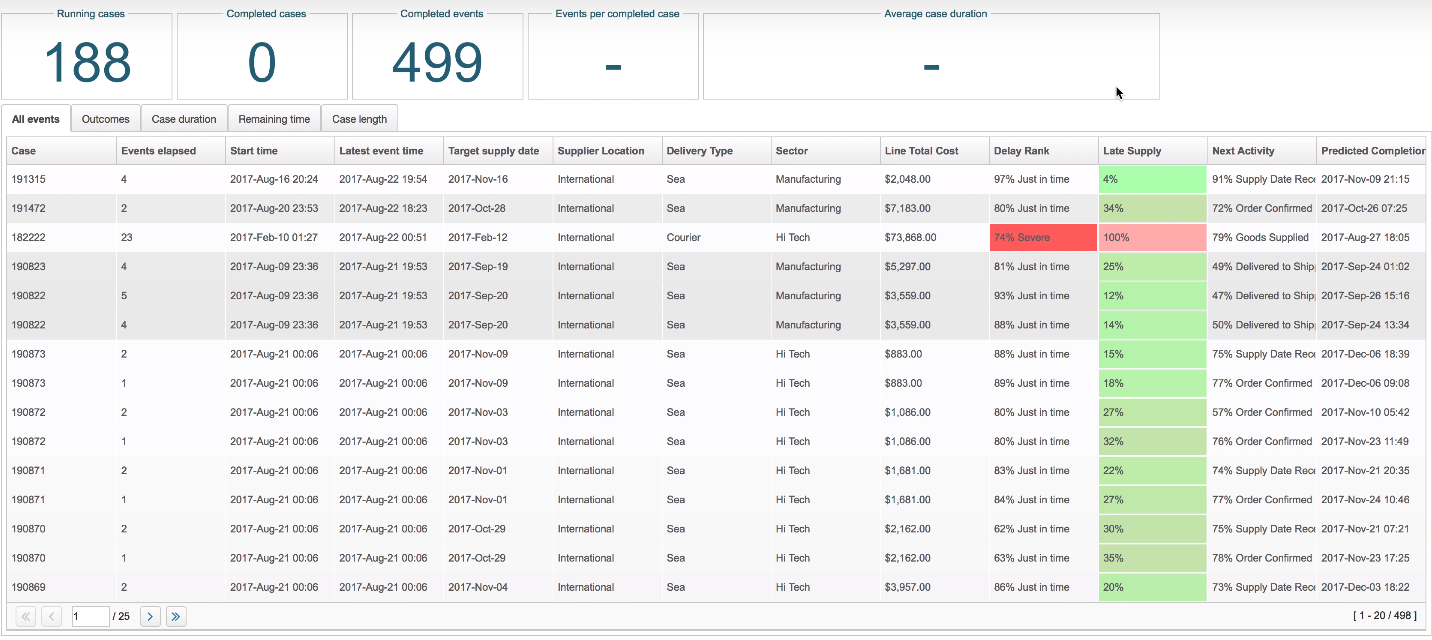
\includegraphics[width=\textwidth]{img/nirdizati-runtime}
	\caption{Main view of the dashboard in the Runtime plugin bundle.}
	\label{fig:nirdizati-runtime}
	\vspace{-\baselineskip}
\end{figure}
%\vspace{-\baselineskip}

Process workers and operational managers can set some process performance targets and subscribe to a stream of warnings and alerts generated whenever these targets are predicted to be violated. Thus, they will be capable of making informed, data-driven decisions to get a better control of the process executions. This is especially beneficial for processes where process participants have more leeway to make corrective actions (for example, in a lead management process).

\section{Conclusion} \label{sec:conclusion}
Through the integration with Nirdizati, Apromore offers a configurable full-stack Web tool that supports users in selecting and tuning various prediction models, and that enables the continuous prediction of different process performance indicators at runtime. Predictions can be presented visually in a dashboard or exported for periodic reporting.

Video demos of the model training and of the runtime functionality can be found at \url{http://youtu.be/CYwLTKAbF1Q} and at \url{http://youtu.be/Q4WVebqJzUI} respectively. The source code is available under the LGPL version 3.0 license at \url{https://github.com/apromore/ApromoreCode}.
%\vspace{-\baselineskip}
\bibliographystyle{splncs03}
\bibliography{paper}

\end{document}
